\chapter{Clustering}

In the exercises in this chapter you will first use a visualization of the k-means clustering that helps to understand how it works. You will then apply the k-means clustering as a machine learning method to segment plants based on their color.

\section{K-means clustering}

Open the file {\tt Visualizing K-Means Clustering.html} from the folder {\tt 01-k-means-visualization}. The applet allows you to see the k-means clustering at work. You can select different strategies for the initial mean-values and different data--sets. You can follow the k-means algorithm step by step. 

Run the k-means algorithm with different initialization strategies and on different data--sets and answer the following questions.

\begin{enumerate}
\item What influence do you think the selection of the initial mean values has on the clustering result ?
\begin{verbatim}







\end{verbatim}
\item Does the k-means algorithm always converge, i.e. does it always come to a point where further iterations do not change the result anymore?
\begin{verbatim}


\end{verbatim}
\item Is the result of the clustering always the same, no matter what the choice of the initial means is?
\begin{verbatim}


\end{verbatim}
\item Does the k-means clustering work as expected on the {\tt Smiley Face} data--set? What is the reason it does or does not work as expected?
\begin{verbatim}









\end{verbatim}
\end{enumerate}

\section{Using K-means clustering for color segmentation}

Images of Arabidopsis thaliana are taken in regular intervals. The aim is to measure the speed with which the area of the rosette of leaves augments under different conditions and treatments. You will use k-means clustering to segment the rosettes of the plants. The tool use the {\tt Color clustering} tool from {\tt FIJI} which comes with the {\tt Weka} machine learning software.   

\begin{figure}[!htb]
 \centering
 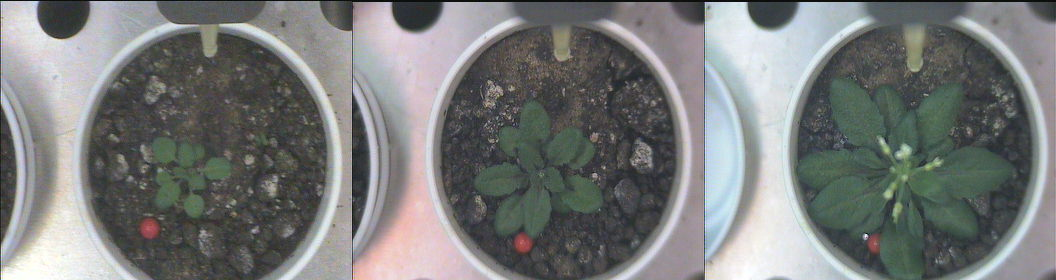
\includegraphics[width=8cm]{arabidopsis}
 \caption{An arabidopsis plant at 3 different stages.}
 \label{figure:arabidopsis}
\end{figure}

\begin{enumerate}
\item Run {\tt FIJI} and open one of the images from the folder {\tt 03 - plants}. Open the {\tt Color clustering} tool from the menu {\tt Plugins>Segmentation>Color Clustering}.
\begin{figure}[!htb]
 \centering
 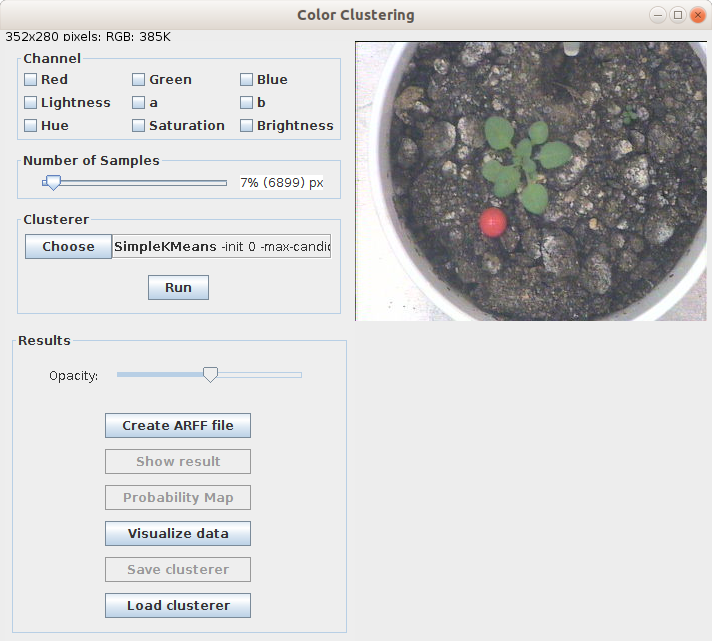
\includegraphics[width=8cm]{color_clustering}
 \caption{The color clustering tool.}
 \label{figure:color_clustering}
\end{figure}
\item How many clusters do you think are appropriate? 
\begin{verbatim}
Number of clusters:

\end{verbatim}
Configure the k-means algorithm to use the number of clusters you have decided to use. Click on the field {\tt SimpleKMeans} to open the options-dialog of the algorithm. Set the number of clusters in the field {\tt numClusters}. You can also change the initialization strategy.

\item Reduce the {\tt Number of Samples}, select one or more features and run the k-means clustering. Note that you can mix features from different color spaces. Experiment with different settings until you obtain a reasonable segmentation of the plant.

\item 
Display the result image and the probability map. The value of a pixel in the result image corresponds to the cluster to which the color of the pixel belongs. The {\tt Probability Map} shows a stack of images, one slice for each cluster. 

What is the class of the color values belonging to the plant?
\begin{verbatim}
Class of plant:

\end{verbatim}
What is the class of the color values belonging to the small red reference object in the form of a ball?
\begin{verbatim}
Class of reference object:

\end{verbatim}

\item Create a selection (roi) from the result of the pixel classification and display it on the original input image. How good is the selection? Measure the area of the surface of the plant.
\begin{verbatim}
Area of the plant:

\end{verbatim}
\item Check the log--window. The clustering algorithm has written information about the clustering into the log--window. Redo the clustering using the features {\tt a} and {\tt b} of the CIELab color space. Find out the number of the cluster corresponding to the plant and find the following information in the log:
\begin{verbatim}
Starting point of the cluster:
Final cluster mean a:
Final cluster mean b:
Size of the training data-set:
\end{verbatim}
\item Visualize the data! The first three fields allow to select the data displayed on the x-- and y--axis and coded a color. Display the a--feature on the X and the b--feature on the Y axis. Let the color represent the cluster. You can change the display-colors of the clusters by clicking on the name of the cluster in the lower part of the window. Set the color of the cluster corresponding to the plant to green. If another cluster was already displayed in green set  it to a different color.
How well separated are the green points from the other points?

\begin{figure}[!htb]
 \centering
 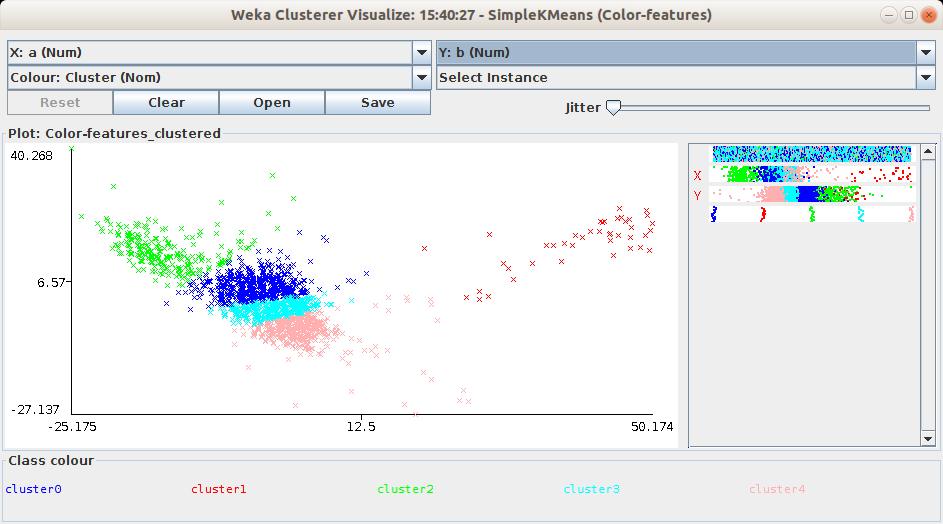
\includegraphics[width=8cm]{cluster_visualization}
 \caption{Visualization of the clusters.}
 \label{figure:cluster-visualization}
\end{figure}

\item Run the clustering again and use only the a--feature this time. Control the resulting segmentation and check the points in the data--visualization. Is the result better or worse than before?
\begin{verbatim}



\end{verbatim}
\end{enumerate}

